
%-------------------------------------------------------------
%				Preparazione wordpress
%-------------------------------------------------------------

\mcchap{Preparazione dell'ambiente di sviluppo per Wordpress}{cap:Preparazione dell'ambiente di sviluppo}

Wordpress, essendo un Content Management System open source, è altamente personalizzabile e dispone
di un innumerevole quantità di \emph{plugin}, gratuiti e a pagamento, per ogni tipo di funzionalità.

Al mio arrivo veniva usata un'installazione base di Wordpress con la sola aggiunta di un plugin chiamato \emph{Microsoft Azure 
for Wordpress} che fa in modo che tutte le immagini che vengono caricate dal pannello di admin di Wordpress
vengono caricate e servite da un server di Microsoft Azure.

Questo serve principalmente, come accennato precedentemente, ad oscurare il dominio del server di Wordpress,
infatti se in una pagina del KN fossero linkate le immagini con l'URL di Wordpress questo potrebbe 
comportare dei problemi di sicurezza.

Per iniziare i miei lavori su Wordpress era necessario impostare un ambiente di sviluppo e dei modi per automatizzare
la distribuzione delle modifiche.

Inoltre era necessario aggiungere un sistema di versionamento che fino a quel momento per Wordpress, a differenza
degli altri progetti, non veniva utilizzato.

\section{Architettura per lo sviluppo}

In 7Pixel per lo sviluppo di tutte le applicazioni, come tipico delle aziende che fanno sviluppo agile, viene usata la seguente architettura basata su tre macchine:
\begin{itemize}
\item {\bf Macchina di produzione}: è la macchina da cui vengono servite l'applicazione per l'utente finale.
\item {\bf Macchina di LAB}: è un ambiente identico a quello di produzione. Viene utilizzato per testare le nuove funzionalità
prima di venire deploiate in produzione.
\item {\bf Macchina di sviluppo}: è la macchina dove lavorano gli sviluppatori, non vengono usati dati reali per i prodotti, 
ma solo un numero ridotto di prodotti fake utili ai fini di testing.
\end{itemize}

\section{Procedura di deploy}
Per la distribuzione delle modifiche si usa il seguente procedura
\begin{itemize}
\item {\bf Sviluppo in locale}: viene editato il codice per aggiungere una nuova funzionalità usando
Test Driven Development, una volta visto in locale che la funzionalità è stata implementata correttamente si passa alla fase successiva
\item {\bf Test in lab}: le nuove modifiche vengono deploiate in LAB, qui, sfruttando un ambiente simile a quello di 
produzione, vengono fatti ulteriori controlli, se si riscontra qualche problema si ritorna alla fase precedente e si corregge
altrimenti si passa alla fase successiva 
\item {\bf Deploy in produzione}: una volta effettuati i controlli in LAB le modifiche vengono pubblicate sulle macchine
di produzione e saranno disponibili agli utenti finali. 

Nei minuti successivi si tiene sotto controllo {\bf New Relic}, un
applicazione di monitoraggio degli errori, per vedere se le modifiche pubblicate fanno generare degli errori inaspettati.
In caso di errori si fa \emph{rollback} alla versione precedente altrimenti la nuova funzionalità viene considerata pubblicata con successo
\end{itemize}

Prima dei deploy, sia in LAB che in produzione, vengono fatti girare tutti i test, unitari e di integrazione, e il codice viene pubblicato solo se tutti questi sono \emph{verdi}, ovvero passano correttamente.

\section{Impostazione della macchine di sviluppo}

Prima del mio arrivo il Team Iguana non si occupava dello sviluppo di Wordpress, non era quindi presente
l'applicazione nelle macchine di sviluppo locale.

È stato mio compito quindi, prima di iniziare a sviluppare, di installare su tutte le macchine di sviluppo
un istanza di Wordpress, servita dal server Nginx\cite{NGINX}, lo stesso server già presente nelle macchine locali per
la reindirizzazione delle chiamate a Kiruby.

È stata poi creata un repository di git per il versionamento di Wordpress. 
Alla radice della cartella \emph{wordpress} (vedi Figura \ref{fig:wptree}) troviamo alcuni file di configurazione e le cartelle \emph{wp-content}, \emph{wp-admin} e \emph{wp-includes}\cite{WPDIR} di queste solo la
cartella \emph{wp-content} viene versionata perchè qui troviamo tutti i file rilevanti per la programmazione delle varie funzionalità, mentre nelle
altre cartelle troviamo file di configurazione e altre funzionalità standard di \emph{wordpress} che non vengono modificati dagli sviluppatori
e rimangono intatte in tutte le macchine.

\begin{figure}
  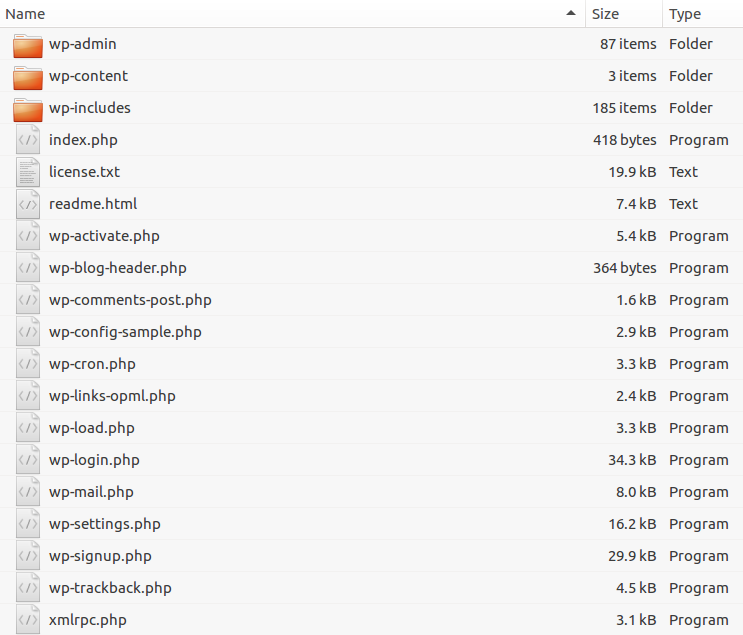
\includegraphics[width=\textwidth]{figure/wpfolder.png}
  \caption{Contenuto della cartella "wordpress".}
  \label{fig:wptree}
\end{figure}

\section{Creazione dello script di deploy}
Lo script di deploy, essendo tutte la macchine di sviluppo e produzione macchine Linux, è stato scritto in un file eseguibile
\emph{kirCMS-autodeploy.sh} utilizzando il linguaggio Bash ed utilizza una procedura simile allo script di deploy 
utilizzato da Kiruby.

Prima di eseguire il deploy è necessario fare commit sul master della repository di Wordpress in modo da avere i sorgenti git aggiornati.

Una volta committate le modifiche da pubblicare bisogna eseguire lo script \emph{kirCMS-autodeploy.sh} passandogli come argomento
\emph{lab} o \emph{pro} a seconda della macchina su cui si vuole deploiare.

Lo script per prima cosa chiede le credenziali di autenticazione, apre un tunnel verso la macchina dove si vuole deploiare e si collega a questo in remoto.

Una volta collegato in remoto viene scaricata da \emph{Gitlab} l'ultima versione committata della repository dentro la cartella /tmp
della macchina e vengono eseguiti tutti i test di PhpUnit eseguendo lo script presente all'interno della repository \emph{test.sh}.

Se i test falliscono viene stampato a console un messaggio con lo stack dell'errore e la procedura termina, lasciando invariata
la versione precedentemente pubblicata.

Se tutti i test passano la cartella scaricata in /tmp viene spostata dentro wordpress col nome wp-content e il server inizierà a
utilizzare le ultime modifiche, la precedente cartella wp-content viene rinominata come wp-content-bkp, la precedente cartella wp-content-bkp
viene eliminata.

La cartella emph{wp-content-bkp} serve a tenere ancora disponibile la versione precedente semplificando la precedura per un eventuale rollback. 

Se vengono individuati degli errori con il nuovo deploy, per ritornare alla situazione precedente è sufficente eliminare la cartella wp-content
e rinominare wp-content-bkp in wp-content.

\begin{verbatim}
	$ cd /media/www/wordpress 
	$ rm wp-content && mv wp-content-bkp wp-content
\end{verbatim}
\emph{comandi da eseguire a terminale per effettuare rollback alla versione precedente}

\newpage 

\begin{lstlisting}[language=bash,caption={Script di deploy: kirCMS-autodeploy.sh}]
#!/bin/bash

set -e

RED_COLOR=`tput setaf 1`
GREEN_COLOR=`tput setaf 2`
RESET_COLOR=`tput sgr0`

CHECKOUT_DIR=wpkiruby
TARFILE=wpkiruby.tar.gz
TARGET_DIR=/media/www/wordpress
WP_CONTENT=wp-content
WP_CONTENT_BKP=wp-content-bkp
UPLOADS=wp-content/uploads

LOGFILE=/media/www/wordpress/wp-content/themes/basic/test/.log.txt
LOAD=/media/www/wordpress/wp-load.php
TESTS=/media/www/wordpress/wp-content/themes/basic/test/.



#CHIEDI USERNAME E CONTINUA DOPO AVER APERTO IL TUNNEL
if [ ! "$1" ]
then
    echo "${RED_COLOR}Dimmi dove vuoi deployare! LAB \
    o PRO?${RESET_COLOR}"
    exit
fi
echo -n "Username: "
read username
gnome-terminal -e "$1.sh $username" 2>&1 > /dev/null &
echo "${GREEN_COLOR}Tunnellizzati e premi un tasto \
per continuare${RESET_COLOR}"
read

#SCARICA LA REPO DA GIT, COMPRIME E MANDA DOVE APERTO IL TUNNEL
cd /tmp && git clone git@gitlab.p7intranet.it:wpkiruby.git

tar -czvf $TARFILE $CHECKOUT_DIR
scp -P 20059 /tmp/${TARFILE} root@localhost:${TARGET_DIR}

rm $TARFILE
rm -rf $CHECKOUT_DIR

echo "${GREEN_COLOR}=== ${TARFILE} copied in remote at \
${TARGET_DIR} ===${RESET_COLOR}"

echo "=== switch WP-CONTENT and create WP_CONTENT_BKP ==="
#COLLEGA AD HOST REMOTO
ssh -C -l root -p 20059 -o UserKnownHostsFile=/dev/null -o \
StrictHostKeyChecking=no -R 8765:192.168.254.140:22 localhost \ 
-i /home/xpuser/shoppydoo/kiruby/key.ssh -t << HERE
    #ESEGUE IN REMOTO
    cd /media/www/wordpress; bash --login
    tar -xzf ${TARFILE}
    [ -d $WP_CONTENT_BKP ] && rm -rf $WP_CONTENT_BKP
    rm ${TARFILE}
    mv $WP_CONTENT $WP_CONTENT_BKP && mv $CHECKOUT_DIR \
    $WP_CONTENT
    chmod 777 -R $UPLOADS
    #ESEGUE I TEST E STAMPA ESITO IN FILE DI LOG
    phpunit --bootstrap $LOAD $TESTS > $LOGFILE
    if grep -q 'OK (' $LOGFILE;
    then
        echo '${GREEN_COLOR}All tests passed!!;
    else
        echo '${RED_COLOR}Tests not passed!! :(';
        cat $LOGFILE; echo '${RESET_COLOR}';
        rm -rf $WP_CONTENT && mv $WP_CONTENT_BKP \
        $WP_CONTENT;    
    fi
HERE
    echo "${GREEN_COLOR} Success, CMS is online!${RESET_COLOR}"
\end{lstlisting}